
%----------------------------------------------------------------------------------------
%   PACKAGES AND OTHER DOCUMENT CONFIGURATIONS
%----------------------------------------------------------------------------------------

\documentclass[paper=a4, fontsize=11pt]{scrartcl} % A4 paper and 11pt font size

\usepackage[T1]{fontenc} % Use 8-bit encoding that has 256 glyphs
\usepackage{fourier} % Use the Adobe Utopia font for the document - comment this line to return to the LaTeX default
\usepackage[english]{babel} % English language/hyphenation
\usepackage{amsmath,amsfonts,amsthm} % Math packages
\usepackage[utf8]{inputenc}
\usepackage{ tipa }
\usepackage{lipsum} % Used for inserting dummy 'Lorem ipsum' text into the template
\usepackage{verbatim}
\usepackage{hyperref}
\usepackage{sectsty} % Allows customizing section commands
\allsectionsfont{\centering \normalfont\scshape} % Make all sections centered, the default font and small caps
\usepackage{graphicx}
\usepackage{fancyhdr} % Custom headers and footers
\pagestyle{fancyplain} % Makes all pages in the document conform to the custom headers and footers
\fancyhead{} % No page header - if you want one, create it in the same way as the footers below
\fancyfoot[L]{} % Empty left footer
\fancyfoot[C]{} % Empty center footer
\fancyfoot[R]{\thepage} % Page numbering for right footer
\renewcommand{\headrulewidth}{0pt} % Remove header underlines
\renewcommand{\footrulewidth}{0pt} % Remove footer underlines
\setlength{\headheight}{13.6pt} % Customize the height of the header
\usepackage{xcolor}
\numberwithin{equation}{section} % Number equations within sections (i.e. 1.1, 1.2, 2.1, 2.2 instead of 1, 2, 3, 4)
\numberwithin{figure}{section} % Number figures within sections (i.e. 1.1, 1.2, 2.1, 2.2 instead of 1, 2, 3, 4)
\numberwithin{table}{section} % Number tables within sections (i.e. 1.1, 1.2, 2.1, 2.2 instead of 1, 2, 3, 4)

\setlength\parindent{0pt} % Removes all indentation from paragraphs - comment this line for an assignment with lots of text
\usepackage{fancyvrb}
\usepackage{anysize}
\marginsize{2cm}{2cm}{1cm}{1cm}
%----------------------------------------------------------------------------------------
%   TITLE SECTION
%----------------------------------------------------------------------------------------

\newcommand{\horrule}[1]{\rule{\linewidth}{#1}} % Create horizontal rule command with 1 argument of height

\title{   
\normalfont \normalsize 
\textsc{Facultad de Ciencias Exactas, Ingeniería y Agrimensura} \\ [25pt] % Your university, school and/or department name(s)
\horrule{0.5pt} \\[0.4cm] % Thin top horizontal rule
\huge Aprendiendo a pronunciar texto en Inglés \\ % The assignment title
\horrule{2pt} \\[0.5cm] % Thick bottom horizontal rule
}

\author{Jeremías Rodríguez} % Your name

\date{\normalsize\today} % Today's date or a custom date

\begin{document}

\maketitle % Print the title

%----------------------------------------------------------------------------------------
%   PROBLEM 1
%----------------------------------------------------------------------------------------

\section{Introducción}

\par La pronunciación del lenguaje inglés ha sido estudiada extensivamente por linguistas, y mucho es sabido sobre las correspondencias entre letras y los sonidos del habla inglesa, llamados \emph{fonemas}.  El inglés es un lenguaje particularmente difícil de dominar por sus irregularidades en la pronunciación. Por ejemplo, la letra "a" en la palabra "gave" es una vocal larga,  pero no en "have" o "read".\\
\par En este trabajo se busca aplicar varios de los contenidos estudiados en este curso (y el anterior) al problema de convertir texto en inglés a su correspondiente transcripción en fonemas\footnote{El Alfabeto Fonético Internacional es un sistema de notación fonética creado por lingüistas. Su propósito es otorgar, de forma regularizada, precisa y única, la representación de los sonidos de cualquier lenguaje oral. Tiene aproximadamente 107 símbolos básicos, y cada idioma hace uso de un subconjunto particular.}. \\

\begin{figure}[h!]
\centering
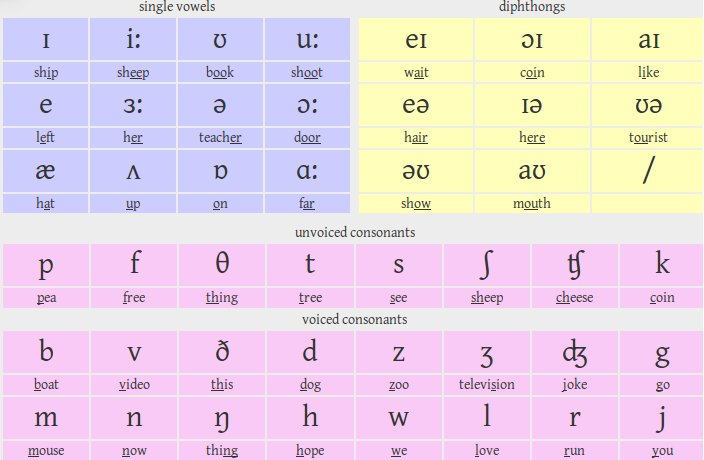
\includegraphics[width=120mm]{phonemicChart.jpg}
\caption{Algunos de los 51 fonemas del inglés oral.}
\label{fig:method}
\end{figure}

\par El dataset utilizado se llama netTalk\footnote{\url{https://archive.ics.uci.edu/ml/datasets/Connectionist+Bench+(Nettalk+Corpus)}}, fue usado por primera vez en el paper  "Parallel Networks that Learn to Pronounce English Text"\cite{parallel}. Los autores entrenaron redes neuronales que convierten strings de texto en inglés (e.g. \textit{calculator}) en strings de fonemas ( $k \ae lkj \omega leIt  \textschwa $).\\
    

\par En este trabajo recrearé y analizaré varios experimentos llevados a cabo en el citado paper (con ANNs). Posteriormente aplicaré otros clasificadores (Random Forest, Gaussian Process, SVM y KNN) y compararé resultados.

\section{Dataset NetTalk}

\subsection{Presentación del dataset}
El dataset netTalk contiene una fila por cada una de las 20000 palabras del \textit{Miriam Webster’s Pocket Dictionary}. Por cada fila, el dataset contiene sólo dos columnas: \\

\begin{center}

\begin{BVerbatim}
[written_representation] [phonemic_representation]
argue                    argY-   
argumentation            argYmxnteS-xn   
argumentative            argYmEntxtIv-   
aright                   xrA--t   
arise                    xrAz-   
aristocracy              @rxstakrxsi   
aristocrat               xrIstxkr@t   
aristocratic             xrIstxkr@tIk   
arithmetic               xrIT-mxtIk   
arithmetical             @rIT-mEtIk-L   
arithmetician            xrIT-mxtIS-xn   
\end{BVerbatim}

\end{center}

Ambas columnas son de tipo string, la primera columna sólo contiene caracteres del alfabeto inglés (abc..z), mientras que la segunda columna contiene caracteres que representan fonemas. Los autores del paper original eligieron un conjunto de 51 fonemas. (ver rawDs/netTalk.names para mas detalle).\\

En el extracto del dataset que he mostrado podemos ver que se ha forzado una correspondencia 1-1 entre letras de la primera columna y fonemas de la segunda: cada fonema corresponde al sonido producido por una de las letras . Por ejemplo, la palabra "arithmetical": 

\begin{center}

\begin{BVerbatim}
a>@ ; r>r ; i>I ; t>T ; h>- ; m>m ; e>E ; t>t; i>I ; c>k ; a>- ; l>l               
\end{BVerbatim}

\end{center}

Los autores del paper original incluyen un fonema "vacío", representado con el símbolo '-', para indicar la ausencia de sonido. Utilizando este simbolo, se completa las transcripciones foneticas para que tengan la misma cantidad de caracteres que la palabra original (lo cual es computacionalmente conveniente).



\subsection{Preprocesamiento}

Todos los métodos que hemos estudiado en Machine Learning y Data Mining requieren que los datos input estén expresados como una matriz numerica. El dataset netTalk que se acaba de introducir es una representación a muy alto nivel de la información que queremos utilizar, y por ello los autores del paper original realizaron una codificación y transformación bastante compleja para obtener datos numéricos con los que trabajar. \\

Comencemos por definir claramente el problema a tratar. Deseamos hallar una función f que convierta strings con palabras en inglés, a strings con su correspondiente transcripción fonética:

\begin{align*}
  f \colon Words &\to Phonetics \\
  f("hypotenuse") &= "hApat-NYs-".
\end{align*}

Utilizando el hecho de que cada letra del input se corresponde a un fonema en el output, podemos reducir el problema a hallar el fonema correspondiente de cada letra. Es decir, deseamos obtener una función $g$ que se focalice en predecir el fonema de una sóla de las letras a la vez, obviamente teniendo en cuenta el entorno de ella. Asumimos que para predecir el sonido de una letra, sólo necesitamos saber las 3 letras anteriores, la letra misma y las 3 siguientes (si las hay):


\begin{align*}
  g \colon L \times L \times L \times L \times L \times L \times L  & \to Phonems \\
  g(-,-,-,\textcolor{red}{h},y,p,o) &= h \\  
  g(-,-,h,\textcolor{red}{y},p,o,t) &= A \\
  g(-,h,y,\textcolor{red}{p},o,t,e) &= p \\
  g(h,y,p,\textcolor{red}{o},t,e,n) &= a \\
  g(y,p,o,\textcolor{red}{t},e,n,u) &= t \\
  g(p,o,t,\textcolor{red}{e},n,u,s)& = - \\
  g(o,t,e,\textcolor{red}{n},u,s,e)& = N \\
  g(t,e,n,\textcolor{red}{u},s,e,-)& = Y \\
  g(e,n,u,\textcolor{red}{s},e,-,-) &= s
\end{align*}

Por supuesto, esta ventana de 7 letras puede no ser suficiente para algunas palabras donde se necesita considerar una porción más amplia para generar una correcta pronunciación; pero en general funciona bien. Finalmente, si obtenemos esta función g, podemos derivar f aplicando sucesivamente g a cada letra del input de f. 

\begin{align*}
  f("hypotenuse") = g("---\textcolor{red}{h}ypo")  g("--h\textcolor{red}{y}pot") g("-hy\textcolor{red}{p}ote") g("hyp\textcolor{red}{o}ten")  \ldots
\end{align*}


Qué ventajas tiene g respecto a f? Al tener un input fijo de 7 caracteres y un output fijo de 1 fonema; podemos aplicar los algoritmos de machine learning que hemos estudiado (tener inputs/outputs de longitud variable complicaria el problema) . Ademas, aprender la función g es sustancialmente más fácil porque sólo se predice un caracter a la vez. \\

Por lo tanto, se convirtió el dataset netTalk a un nuevo dataset de 8 columas, donde dividimos cada palabra en varias filas como se ilustró arriba con "hypotenuse". En nuestro caso, de tener 10000 palabras pasamos a tener 146934 filas. Los scripts utilizados en esta fase pueden verse en /src/encodedDs. \\

El paso restante es codificar todos los caracteres (letras y fonemas) de las 146934 filas como números. Para codificar las \textbf{letras del input} usaremos una representación muy simple: Dado que tenemos 26 letras en el alfabeto inglés, cada letra por 26 columnas binarias 1-0. Si la primera letra era una 'j', entonces la columna 10 tendrá un 1 y las otras 25 columnas un cero. Los \textbf{fonemas output}, por otra parte, se codificarán en 20 columnas binarias (ver anexo I).\footnote{Los 50 fonemas se codifican en 18 columnas que representan "articulatory features" que los definen, como por ejemplo si tienen un tono alto, medio o bajo; si el ruido procede de la garganta, del paladar, etc; o si el ruido es con o sin voz.} \\

Por lo tanto, el dataset final de 146934 filas tendrá 26 * 7 columnas binarias representando las 7 letras input; y otras 18 columnas binarias representando el fonema output. A este dataset resultante le aplicaré distintas técnicas de aprendizaje que estudiamos en el curso.

\section{Redes Neuronales}
El primer paso es repetir los exprimentos que se realizaron usando redes neuronales en \cite{parallel}. Para ello, utilizaré una red neuronal con 26 * 7 neuronas en la capa de entrada, y 18 en la capa de salida. 

\begin{figure}[h!]
\centering
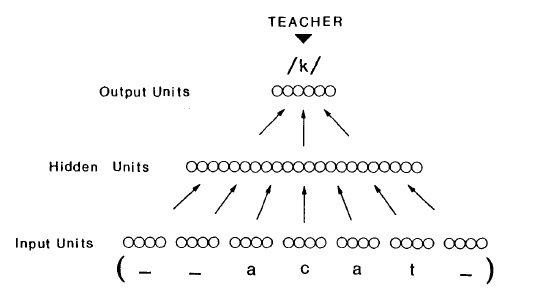
\includegraphics[width=100mm]{figure1.jpg}
\end{figure}


\subsection{Optimización de parámetros}

Para optimizar parametros se usaron 1000 de las 20000 palabras del dataset original; divididas en 750 training y 250 validacion. Realicé la búsqueda en grid search para learning rate ($\eta$) y momentum ($\mu$) entre  $10^{-1} y 10^{-5}$ (25 combinaciones). Utilicé el algoritmo backpropagation, en particular una version modificada del codigo en C que utilizamos en el curso de machine learning. Los parámetros óptimos fueron $\mu$=0.0001 y $\eta$=0.01 y el código de toda esta sección puede verse en /src/ANNs

\begin{comment}
\begin{tabular}{ |c|c|c|c|c|c|  }
\hline
 & $\eta$ =.1 & $\eta$ =.01 & $\eta$ =.001 & $\eta$ =.0001 & $\eta$ =.00001 \\
\hline 
$\mu$ =.1     & 25.4  & 24.85 & 25.06 & 33.52 & 39.01 \\
$\mu$ =.01    & 24.92 & 24.38 & 25.18 & 33.61 & 39.94 \\
$\mu$ =.001   & 25.24 & 24.00 & 25.24 & 33.61 & 39.98 \\
$\mu$ =.0001  & 25.26 & 23.99 & 25.26 & 33.60 & 39.98 \\
$\mu$ =.00001 & 25.26 & 23.99 & 24.84 & 33.60 & 39.98 \\
\hline
\end{tabular}
\end{comment}

\subsection{Resumen de resultados usando ANNs}

\begin{figure}[h!]
\centering
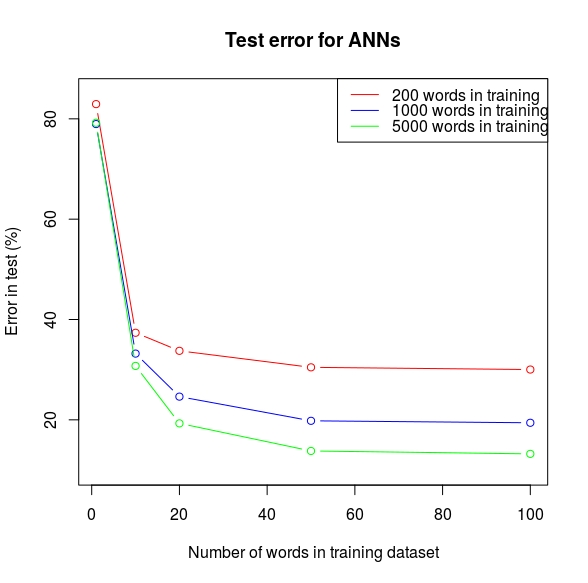
\includegraphics[width=112mm]{annresults.jpg}
\end{figure}

Una vez seleccionados los parámetros óptimos, el siguiente paso fue entrenar redes con distintas cantidades de neuronas intermedias y con distintas cantidades de puntos en training, y los resultados pueden verse en la figura anterior. \\

Algunas apreciaciones:

\begin{itemize}
\item Como vemos, usando una red con 20 o más neuronas podemos llegar a un accuracy realmente alto, donde más del 80\% de los fonemas son generados correctamente.
\item El mejor error en test se obtiene con 5000 palabras en training y 100 neuronas, donde el 86.78\% de los fonemas son generados correctamente.
\item A partir de 50 neuronas en adelante, continuar agregando más neuronas no mejora el resultado. Apartentemente no queda más información que pueda ser aprendida por una ANN llegado a ese punto, independientemente de la complejidad de la red. (Para comprobar esto, entrene una red con 150 neuronas intermedias; y el error no mejoro aun entrenando con muchisimas epocas)
\item Similarmente, la ganancia de seguir agregando más palabras al dataset de entrenamiento se reduce cada vez más a medida que llegamos a unas 5000 palabras. 
\end{itemize}

El "estancamiento" en la reduccion del error (descripto en los ultimos dos items) probablemente se deba a que:

\begin{itemize}
\item Hay irregularidades y excepciones del lenguaje que probablemente no puedan ser aprendidas de otra forma que memorizando los casos puntuales.
\item Estamos usando una ventana de 7 caracteres para pronunciar, y probablemente hay palabras cuyos patrones de pronunciacion podrian ser aprendidos considerando una ventana mayor.
\end{itemize}


Me parece asombroso llegar a predecir con tanta exactitud los fonemas, dado que este problema es muy complejo, altamente dimensional y posee una gran cantidad de reglas y excepciones. \\

Lo que mas me sorprende de estos resultados es que con sólo 200 palabras de ejemplo del idioma somos capaces de predecir la pronunciación del resto del idioma con casi 80\% de precisión (habilidad que a un ser humano puede llevarle realmente mucho tiempo y ejemplos adquirir). \\


\subsection{Ejemplos y conclusión}

Esta tarea exhibe una gran cantidad de regularidades globales junto con reglas más especializadas y casos excepcionales. Los resultados fueron muy buenos y las redes aprendieron exitosamente a generar una pronunciación cercana a la real. Veamos algunos ejemplos:

\begin{center}
\begin{BVerbatim}
Written Representation  predicted Phonetics   real Phonetics  
machine                 m@C-en-               mxS-in-  
learning                lI-rnIG-              l--RnIG- 
unexpected              xnEXpEktxd            xnIXpEktxd  
beautiful               bcc-tIfcl             bY--tIf^l 
telescope               tIlEskxp-             tElxskop- 
virus                   varxs                 vArxs

\end{BVerbatim}
\end{center}


Como se puede apreciar, la red se confunde en varios fonemas, pero los errores son muy similares a los que cometemos las personas, pues la confusión se da generalmente entre vocales con sonidos similares. \\

Me interesaría mucho probar si este mismo procedimiento funcionaría para aprender cualquier idioma, provisto un dataset de palabras y sus transcripciones fonéticas.

\section{ Otros metodos de machine learning }

Me interesa analizar ahora la performance de otros algoritmos que hemos estudiado en el curso, y compararla con los resultados vistos en la seccion anterior. Los metodos que decidi aplicar a este problema de clasificacion son:

\begin{itemize}
\item \textbf{Nearest Neighbor}: Decidi usar este metodo tan simple para obtener un "baseline" del error. En este caso, si deseamos predecir el fonema generado por el input (y,p,o,\textcolor{red}{t},e,n,u), se descartan las columnas de contexto y simplemente se busca en el dataset de training otro input donde la letra a predecir sea tambien \textcolor{red}{t}. Encontrado este nearest neighbor en train, se retorna el fonema asociado.

\item \textbf{Nearest Neighbor silaba}:Similar al anterior. En este caso, si deseamos predecir el fonema generado por el input (y,p,o,\textcolor{red}{t},e,n,u), buscamos el nearest neighbor en train usando las tres columnas centrales (o,\textcolor{red}{t},e). 

\item \textbf{Random Forest}: Dado que hay 18 columnas binarias de output, entrené 18 clasificadores RF, cada uno especializado en predecir la columna de output i-ésima. Utilicé 500 árboles por ensemble.

\item \textbf{SVM}: Al igual que con RF, entrene 18 clasificadores, cada uno especializado en predecir la columna de output i-ésima. Use un kernel Gaussiano, lo cual involucra la dificultad extra de optimizar parametros. Para cada una de las 18 columnas, optimice $C$ y $\sigma$ en grid search.

\item \textbf{Gaussian Processes}: Si bien no estudiamos este metodo en el curso, me parecio interesante incluirlo(add reference). Al igual que para SVM y RF, tuve que entrenar un clasificador por columna. El kernel usado es  Gaussiano, aunque la optimizacion de parametros es realizada automaticamente por kernlab.

\end{itemize}

Para cada uno de estos 5 metodos, repeti los calculos usando datasets de entrenamiento de distinto tamanyo: 200, 1000 y 5000 palabras. Las restantes (19800, 19000 y 15000 respectivamente) fueron usadas para calcular el error discreto en la prediccion de cada fonema.


\newpage

\begin{center}
\begin{figure}[h!]
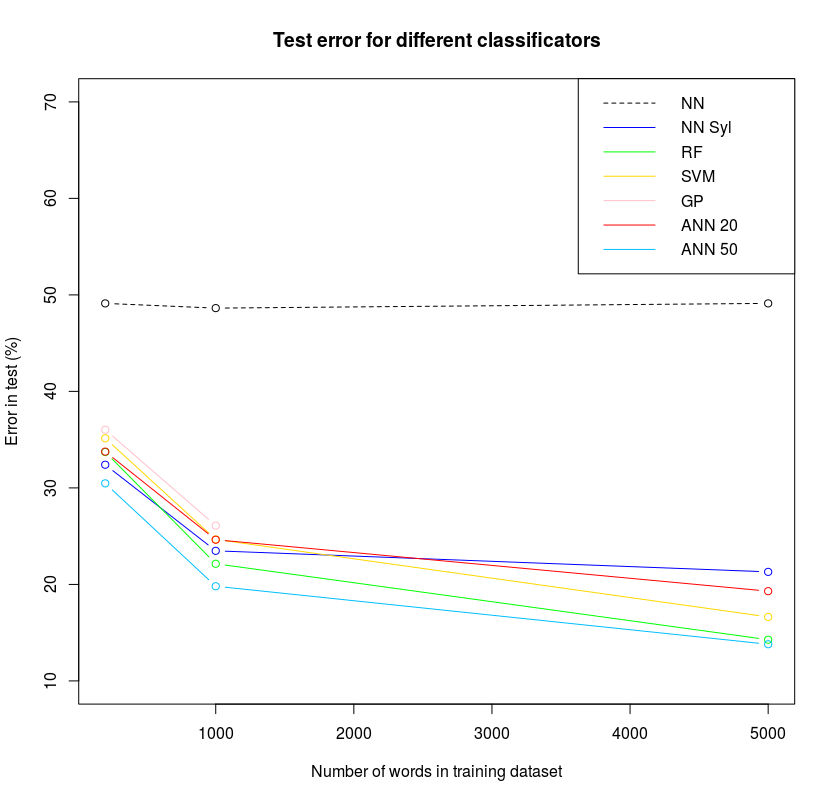
\includegraphics[width=170mm]{figure.png}
\end{figure}
\end{center}

*porque ANNS son mas suitable
*cositas extra de c/metodo

anexo 1: tabla
\begin{thebibliography}{9}
\bibitem{parallel} 
Terrence J. Sejnowski and Charles R. Rosenberg
\textit{Parallel Networks that Learn to Pronounce English Text}. 
Complex Systems 1 (1987)
 

\end{thebibliography}

\end{document}
